%%%%%%%%%%%%%%%%%%%%%%%%%%%%%%%%%%%%%%%%%%%%%%%%%%%%%%%%%% 
% This file examplifys a chapter written in a single file
%%%%%%%%%%%%%%%%%%%%%%%%%%%%%%%%%%%%%%%%%%%%%%%%%%%%%%%%%%

%#!latexmk main.tex
\begin{bibunit}
\setcounter{chapter}{0}
\chapter{Introduction}\label{chap:1}

% abstract
This is citation example~\cite{Einstein1905SR}.
\lipsum[60]

\section{Introduction section 1}\label{sec:1_1}

\lipsum[60]

% example table
\begin{table}[bt]
\centering
\caption{This is an example table.}
\includestandalone[mode=tex]{table/table_1_1}
\label{Table:1_1}
\end{table}


\section{Introduction section 2}\label{sec:1_2}

\lipsum[60]

% example figure
\begin{figure}[htb]
\captionsetup[subfigure]{font={bf,large}, skip=1pt, margin=-0.7cm,justification=raggedright, singlelinecheck=false}
 \centering
  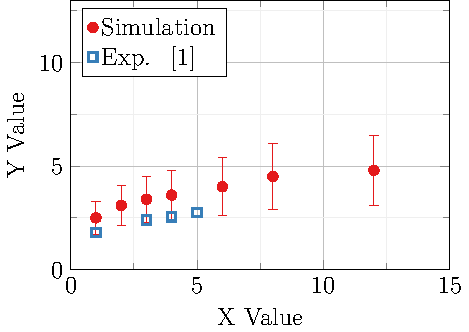
\includegraphics[width=8.6cm]{fig_1_1/fig_1_1.pdf}
  \caption{The example image with citation.}
\label{Fig:1_1}
\end{figure}


\lipsum[60]


\putbib
\end{bibunit}

% if you submit, uncomment the following and comment bibunit
% \input{../../bu1.bbl}